\subsection{Real drift: 40 weeks of CESNET traffic}\label{sec:cesnet}
The injected drift above is a stress test. To check FOA on drift nobody designed, we use
CESNET-TimeSeries24~\cite{cesnet}: traffic statistics of IP addresses in a national research network
from October 2023 to July 2024, which span a semester, holidays and the institutions' own changes. The
fleet is the twelve most active addresses of one institution (they share its network); a learning cycle
is one day of 10-minute aggregates (twelve statistics: flows, packets, bytes, destinations, ports,
protocol and direction ratios, duration, TTL), the first 28 days calibrate, and 252 days stream. Nothing
about the drift is injected. The attack is modelled, because the dataset has no attack labels: the IP's
own traffic turned into a scanner (twenty times the flows, thirty times the destinations, short flows),
with a boundary poisoner from day 30. Eleven of the twelve addresses meet the victim rule.

The real drift is milder than our stress test: the static detector stays at \CesStaticFPR\ false
alarms, except one address whose behaviour changes for good in the second half and which every rule
loses. Every adaptive rule pays something for adapting to daily variation (single device \CesAutoFPR,
alarm-rate switch-off \CesKLFPR); FOA pays least among the protected rules (\CesFOAFPR). Under attack,
naive learning was compromised in \CesNaiveComp\ of runs, single-device adaptation and the alarm-rate
switch-off in \CesAutoComp\ and \CesKLComp, the frozen reserve in \CesFrozenComp, and FOA in
\CesFOAComp\ (Figure~\ref{fig:cesnet}).

\begin{figure*}[t]
\centering
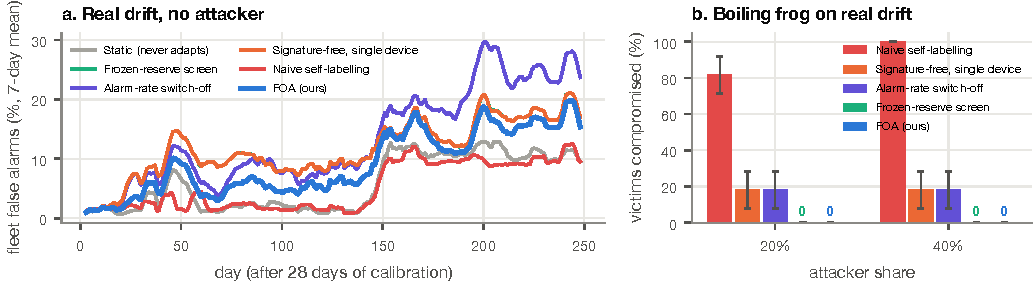
\includegraphics[width=\textwidth]{figures/fig_cesnet.pdf}
\caption{CESNET-TimeSeries24, twelve addresses of one institution, one learning cycle per day.
(a) Fleet false alarms under real drift, no attacker (the frozen reserve never filters here and coincides with single-device adaptation). (b) Victims compromised by a boundary poisoner
(11 victims, 5 held-out seeds).}
\label{fig:cesnet}
\end{figure*}
